\section{Regressão Linear}
O principal objetivo por trás da regressão linear é de estimar um valor $y \in \Re$ dado uma característica $x$.
Por exemplo, pode se estimar o valor de um estoque no dia seguinte de acordo com as vendas dos dias anteriores, os batimentos cardíacos de um atleta de acordo com a distância que percorreu, entre outras aplicações \cite{smola2008introduction}. 
 
 A Figura 1 mostra um bom exemplo de um método de regressão linear. Os pontos na figura são amostras obtidas das características $x$ da base de dados, o objetivo é criar uma função $f(x)$ que se aproxime da melhor forma dos valores observados.
\begin{figure}[H]
	\label{reg}
	\begin{centering}
		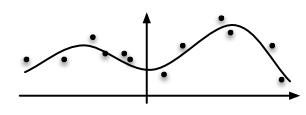
\includegraphics[width = 300pt]{img/regressao.png}
		\caption{Exemplo de regressão linear}
	\end{centering}	
	
\end{figure}

A função $f(x)$ utilizada pode ser representada pela forma:

$$ f(x) = b_0 + b_1*x_1 + b_1*x_1 + b_2*x_2 + ... + b_n*x_n $$

onde $x_{1,2,..n}$ correspondem às características da base de dados utilizada, $b_0$ corresponde à constante e $b_{1,2,..n}$ são os coeficientes. Os dois últimos são termos que o o método de regressão linear irá ajustar de forma a obter uma função que se aproxime dos valores dados pelo conjunto de treinamento.

Abaixo o código em linguagem python do processo de aprendizado da base de dados:
\begin{lstlisting}[language = python, numbers = left, ,backgroundcolor = \color{yellow!20}]
# Importing the libraries
import numpy as np
import pandas as pd

# Lista de Parametros
RATIO_TESTE_TREINO = 1000/3168
rs = np.random.randint(0,100)


#Importando a base de dados
dataset = pd.read_csv('voice.csv')
X = dataset.iloc[:, :-1].values
y = dataset.iloc[:, 20].values

#  Transformando as labels em numeros
from sklearn.preprocessing import LabelEncoder, OneHotEncoder
labelencoder_y = LabelEncoder()
y = labelencoder_y.fit_transform(y)
onehotencoder = OneHotEncoder(categorical_features = [0])
y = onehotencoder.fit_transform(y).toarray()
y = np.transpose(y)

# Dividindo a base de dados em treinamento e teste
from sklearn.cross_validation import train_test_split
X_train, X_test, y_train, y_test = train_test_split(X,y,test_size=RATIO_TESTE_TREINO, stratify=y)

# Metodo de regressao linear simples
from sklearn.linear_model import LinearRegression
regressor = LinearRegression()
regressor.fit(X_train, y_train)

#Prevendo os resultados da base de testes
y_pred = regressor.predict(X_test)
y_pred = np.round(y_pred)

#Calcular a precisao dos resultados
from sklearn.metrics import accuracy_score
print('Accuracy simple linear regression: %.2f\n' % accuracy_score(y_test, y_pred))
\end{lstlisting}  

Com uma base de treinamento de 2000 instâncias e uma base de treino de 1 168 instâncias, a precisão desse método foi entre 96\% e 97\%.